%! TEX root = ../main.tex
% ==============================================================
% IMMUTABLE — generated automatically, do not edit this block
%
% — Provenance ───────────────────────────────────────────────────
%   script            : analysis_scratch/wind_doppler_arrival_shift.py
%   computed_in       : analysis_scratch/wind_doppler_arrival_shift.py (pre-paddle window 0–25 s, eta vs t at all 3 probes; compares wind-wave background at upstream IN probes vs panel-shadowed OUT probe)
%   plot_type         : pre_paddle_overlay
%   data_class        : DELEG
%   generated_at      : 2026-05-12T09:46:44
%   findings_doc      : memory/methodology_wind_enhances_A_in.md
%
% — Thesis context ──────────────────────────────────────────────
%   chapter           : 04
%   caption_label     : fig:ch04_wind_pre_paddle_overlay
%   caption_short     : Vindsignal før padlestart
%
% — Filters ────────────────────────────────────────────────────
%   panel             : full
%   wind              : no, full
%   amplitude [V]     : 0.2
%   frequency [Hz]    : 1.3
%   probes            : 
%   run_category      : 
%   quality_flag      : ok
%   mooring           : 
%
% — Data provenance ────────────────────────────────────────────
%   n_runs            : 
%   in_probes_used    : 
%   out_probes_used   : 
%   probe_configs     : 
%   non_final_config_n: 
%   datasets        :
%     (none registered — set plot_utils.ACTIVE_DATASETS)
%   run_paths       :
%     (omitted — aggregate over > threshold runs, see datasets)
%
% — Method / numerical parameters ─────────────────────────────
%   grouper           : 
%   collapse_panels   : 
%   fft_window_hz     : 
%   extra_params      : runs: nw=/Users/ole/Kodevik/wave_project/wavedata/20260327-ProbePos4_31_FPV_2-tett6roof-under9Mooring30-height100-lowrange/fullpanel-nowind-amp0200-freq1300-per240-depth580-mstop30-run1.csv, fw=/Users/ole/Kodevik/wave_project/wavedata/20260326-ProbePos4_31_FPV_2-tett6roof-under9Mooring-height100-lowrange/fullpanel-fullwind-amp0200-freq1300-per240-depth580-mstop30-run1.csv. plot covers t ∈ (0, 25 s) — entire pre-paddle + chirp + first arrival. vertical dotted line per panel = r/c_g(f) for that probe.
%
% — Summary stats cited in caption ────────────────────────────
%   (none registered — pass extra_stats=... to build_fig_meta)
%
% — Subfigures available ───────────────────────────────────────
%     FIGURES/ch04_wind_pre_paddle_overlay.pdf
% ── end immutable block ─────────────────────────────────────────
\begin{figure}[htbp]
  \centering
  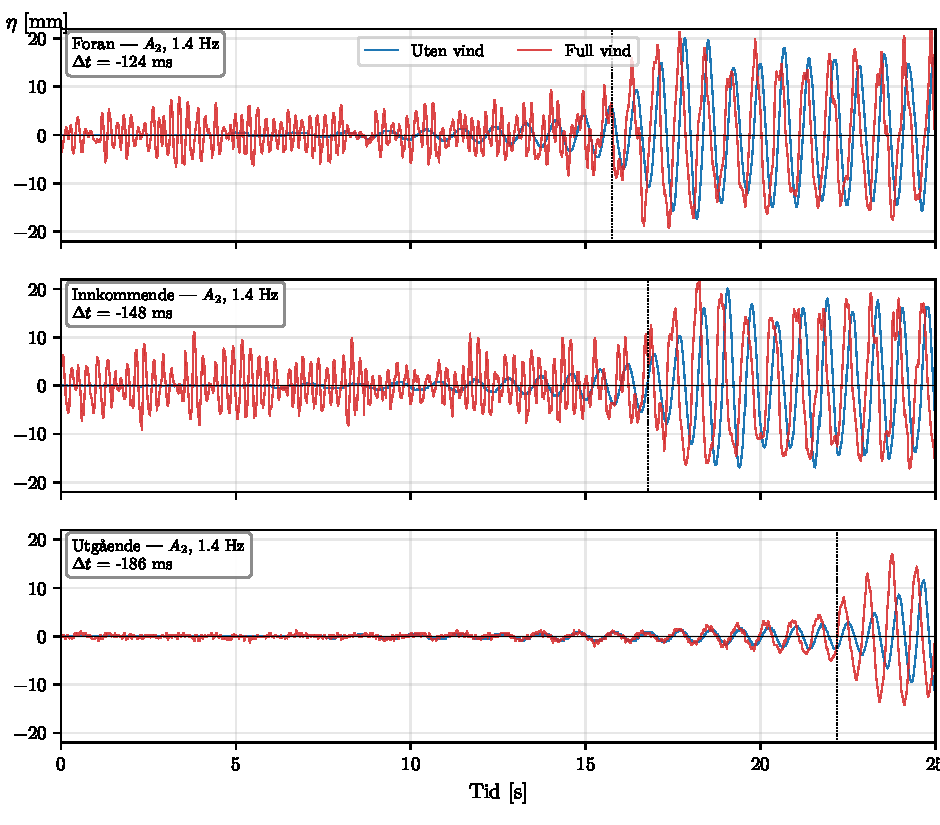
\includegraphics[width=\linewidth]{FIGURES/ch04_wind_pre_paddle_overlay.pdf}
% >>> CAPTION-SYNC START (do not edit this block; sync_captions.py overwrites)
  \caption[Vindsignal før padlestart]{
    To like bølger, med og uten vind, lagt oppå hverandre.
  }
% <<< CAPTION-SYNC END
  \label{fig:ch04_wind_pre_paddle_overlay}
\end{figure}
